\section{eo\-SSGAStoch\-Tournament\-Replacement$<$ EOT $>$ Class Template Reference}
\label{classeo_s_s_g_a_stoch_tournament_replacement}\index{eoSSGAStochTournamentReplacement@{eoSSGAStochTournamentReplacement}}
SSGA stochastic tournament replacement.  


{\tt \#include $<$eo\-Reduce\-Merge.h$>$}

Inheritance diagram for eo\-SSGAStoch\-Tournament\-Replacement$<$ EOT $>$::\begin{figure}[H]
\begin{center}
\leavevmode
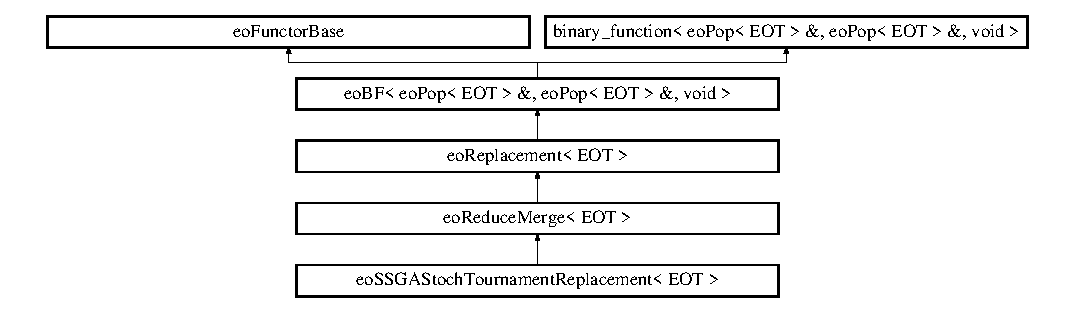
\includegraphics[height=3.76344cm]{classeo_s_s_g_a_stoch_tournament_replacement}
\end{center}
\end{figure}
\subsection*{Public Member Functions}
\begin{CompactItemize}
\item 
{\bf eo\-SSGAStoch\-Tournament\-Replacement} (double \_\-t\_\-rate)\label{classeo_s_s_g_a_stoch_tournament_replacement_a0}

\end{CompactItemize}
\subsection*{Private Attributes}
\begin{CompactItemize}
\item 
{\bf eo\-Stoch\-Tournament\-Truncate}$<$ {\bf EOT} $>$ {\bf truncate}\label{classeo_s_s_g_a_stoch_tournament_replacement_r0}

\item 
{\bf eo\-Plus}$<$ {\bf EOT} $>$ {\bf plus}\label{classeo_s_s_g_a_stoch_tournament_replacement_r1}

\end{CompactItemize}


\subsection{Detailed Description}
\subsubsection*{template$<$class EOT$>$ class eo\-SSGAStoch\-Tournament\-Replacement$<$ EOT $>$}

SSGA stochastic tournament replacement. 

Is an {\bf eo\-Reduce\-Merge}{\rm (p.\,\pageref{classeo_reduce_merge})}. It much cleaner to insert directly the offspring in the parent population, but it is NOT equivalent in case of more than 1 offspring as already replaced could be removed , which is not possible in the {\bf eo\-Reduce\-Merge}{\rm (p.\,\pageref{classeo_reduce_merge})} So what the heck ! 



Definition at line 108 of file eo\-Reduce\-Merge.h.

The documentation for this class was generated from the following file:\begin{CompactItemize}
\item 
eo\-Reduce\-Merge.h\end{CompactItemize}
